%
% Annual Cognitive Science Conference
% Sample LaTeX Paper -- Proceedings Format
%
% Original : Ashwin Ram (ashwin@cc.gatech.edu)       04/01/1994
% Modified : Johanna Moore (jmoore@cs.pitt.edu)      03/17/1995
% Modified : David Noelle (noelle@ucsd.edu)          03/15/1996
% Modified : Pat Langley (langley@cs.stanford.edu)   01/26/1997
% Latex2e corrections by Ramin Charles Nakisa        01/28/1997
% Modified : Tina Eliassi-Rad (eliassi@cs.wisc.edu)  01/31/1998
% Modified : Trisha Yannuzzi (trisha@ircs.upenn.edu) 12/28/1999 (in process)
% Modified : Mary Ellen Foster (M.E.Foster@ed.ac.uk) 12/11/2000
% Modified : Ken Forbus                              01/23/2004
% Modified : Eli M. Silk (esilk@pitt.edu)            05/24/2005
% Modified : Niels Taatgen (taatgen@cmu.edu)         10/24/2006
% Modified : David Noelle (dnoelle@ucmerced.edu)     11/19/2014

%% Change ''letterpaper'' in the following line to ''a4paper'' if you must.

\documentclass[10pt,letterpaper]{article}

\usepackage{cogsci}
\usepackage{pslatex}
\usepackage{apacite}
\usepackage{amsmath,amssymb}
\usepackage{graphicx}
\usepackage{subcaption}
\usepackage{color}
\usepackage{url}
\usepackage{todonotes}
\usepackage{mathtools}
\usepackage{stmaryrd}
\usepackage{booktabs}
\usepackage{array}
\graphicspath{{./figures/}}

%\newcommand{\url}[1]{$#1$}

\definecolor{Red}{RGB}{178,34,34}
\definecolor{Green}{RGB}{10,200,100}

\newcommand{\red}[1]{\textcolor{Red}{#1}}
\newcommand{\rdh}[1]{\textcolor{Red}{rdh: #1}}
\newcommand{\denote}[1]{\mbox{ $[\![ #1 ]\!]$}}
\newcommand{\subsubsubsection}[1]{{\em #1}}
\newcommand{\eref}[1]{(\ref{#1})}
\newcommand{\tableref}[1]{Table \ref{#1}}
\newcommand{\figref}[1]{Fig.~\ref{#1}}
\newcommand{\appref}[1]{Appendix \ref{#1}}
\newcommand{\sectionref}[1]{Section \ref{#1}}

\title{Graphical convention formation during visual communication}

% \author{\begin{tabular}[htbp]{c@{\extracolsep{1em}}c@{\extracolsep{1em}}c@{\extracolsep{1em}}c} \\
% {\large \bf Robert X. D. Hawkins} & {\large \bf Megumi Sano} & {\large \bf Noah D. Goodman} & {\large \bf Judith E. Fan}\\
% Department of Psychology & Department of Psychology & Department of Psychology & Department of Psychology \\
% Stanford University & Stanford University & Stanford University & UC San Diego \\
% \texttt{rxdh@stanford.edu} & \texttt{megsano@stanford.edu} & \texttt{ngoodman@stanford.edu} & \texttt{jefan@ucsd.edu} \\
% \end{tabular}
% }

\author{\large \bf Anonymous Authors}

\begin{document}
\maketitle

\begin{abstract}
Drawing is a versatile technique for visual communication, ranging between photorealistic rendering from observation and schematic diagrams consisting entirely of symbols. 
How does a medium spanning such a broad range of appearances reliably convey meaning?
A natural possibility is that drawings derive meaning from both their visual properties as well as shared knowledge between people who use them to communicate. 
Here we evaluate this possibility by investigating how the accumulation of shared knowledge via extended visual communication between two people influences the drawings they produce and how well they communicate. 
We developed a drawing-based reference game in which two participants repeatedly communicated about visual objects. 
Across a series of controlled experiments, we found that pairs discover increasingly sparse yet effective ways of depicting them. 
These gains were specific to those objects that were repeatedly referenced, and went beyond what could be explained by task practice or the visual properties of the drawings alone. 
We employed modern techniques from computer vision to characterize how the high-level visual features of drawings changed, finding that drawings of the same object became more consistent within a pair and divergent across different pairs.
Taken together, these findings suggest that visual communication promotes the emergence of depictions whose meanings are increasingly determined by shared knowledge rather than their visual properties alone.

\textbf{Keywords:}
sketch understanding; alignment; drawing; iconicity; visual abstraction

% On each trial, both players were shown an array of objects; the sketcher’s goal was to draw one of these, the target, so that the viewer could guess the target as quickly as possible. 
% The game included two sets of objects: objects in one set were drawn repeatedly, while those in a control set were drawn once at the beginning and again at the end of the game. 
% While we observe gains in communication efficiency for all objects, they were greater for the repeated objects, suggesting both task-level and object-level benefits of repeated communication. 
% Moreover, different pairs discovered different solutions for efficient communication, suggesting the existence of multiple equilibria in the space of viable graphical conventions. 

\end{abstract}

\section{Introduction}

From ancient etchings on cave walls to modern digital displays, visual communication lies at the heart of key human innovations (e.g., mapmaking, data visualization), and forms the foundation for the cultural transmission of knowledge and higher-level reasoning. 
Perhaps the most basic and versatile technique supporting visual communication is drawing, the earliest examples of which date to at least 40,000-60,000 years ago \cite{hoffmann2018u,Aubert:2014jy}, and which has since been adapted to a broad diversity of applications, ranging from photorealistic rendering from observation to schematic diagrams consisting entirely of symbols. 

Even drawings of the same object can be highly variable \cite{quickdraw2017}.
How does a medium spanning such a broad range of appearances reliably convey meaning? 
On the one hand, prior work has found that semantic information in a figurative drawing, i.e., the object it represents, can be derived purely from its perceptual properties \cite{FanCommon2018}. 
On the other hand, other work has emphasized the role of socially-mediated information and context for making appropriate inferences about what even a figurative drawing represents \cite{goodman1976languages,gombrich1969art}.

How can these two perspectives be reconciled? 
Our approach is to consider the joint contributions of visual information and social context in determining how drawings derive meaning \cite{fan2018modeling,abell2009canny}, and to propose that a critical factor affecting the balance between the two may be the amount of shared knowledge between communicators. 
Specifically, we explore the hypothesis that accumulation of shared knowledge via extended visual communication may promote the development of increasingly schematic yet effective ways of depicting a physical object, even as these \textit{ad hoc} graphical conventions may be less readily apprehended by others who lack this shared knowledge. 

To investigate this, we used an online drawing-based reference game in which two players repeatedly communicate about visual objects, and examined both how their task performance and the drawings they produced changed over time. 
Our approach was inspired by a large literature that has documented the benefits of extended interaction for facilitating communication in several modalities, including language \cite{ClarkWilkesGibbs86_ReferringCollaborative,HawkinsFrankGoodman17_ConventionFormation}, gesture \cite{goldin1996silence,fay2014creating}, and drawings \cite{garrod_foundations_2007,fay2010interactive}.

% extra: Galantucci:2005uh,healey2007graphical,theisen2010systematicity 

%% jefan: I want another sentence here, if possible, stating the limitations of this prior work that sets up the contributions of the current paper better.

There are three aspects of the current work that advances our prior understanding: \emph{first}, we include a control set of objects that were not repeatedly drawn, allowing us to measure the specific contribution of repeated reference; \emph{second}, we measure how strongly the visual properties of drawings drive recognition in the absence of interaction history, while equating other task variables; and \emph{third}, we employ recent advances in computational vision to quantitatively characterize changes in the high-level visual properties of drawings across repetitions. 

\section{Part I: How does repeated reference support successful visual communication?}

%% intro to this section
% \rdh{eventually need to compress these methods quite a bit (participants can be 1 sentence, much less detail about stim selection and procedure, etc.)} 

Our first goal was to understand how repeated visual communication about an object influences how they well  people communicate about that object.  
To accomplish this, we developed a drawing-based reference game for two players. 
On each trial, both players were shown a set of four objects; the sketcher’s goal was to draw one of these, the target, so that the viewer could guess the target as quickly as possible. 
The game included two sets of objects: objects in one set were drawn repeatedly, while those in a control set were drawn once at the beginning and again at the end of the game.
We hypothesized that repeated visual reference to a visual object would lead to more efficient communication about that object, relative to control objects. 

% gains in communication efficiency for all objects, they were greater for the repeated objects, suggesting both task-level and object-level benefits of repeated communication.

% Our goal was to investigate how the accumulation of shared knowledge via extended visual communication between two people influences the drawings they produce and how well they communicate. 
% Towards this end, we developed a visual communication task in which people repeatedly referred to familiar objects, but where pre-existing graphical conventions were unlikely to be sufficient to succeed. 
% In line with prior studies of repeated verbal communication \cite<e.g>{ClarkWilkesGibbs86_ReferringCollaborative} and visual communication about verbal stimuli \shortcite<e.g.>{garrod_foundations_2007}, we hypothesized that repeated visual reference to a visual object would lead to more efficient communication about that object.
% Departing from prior studies, our experiment critically includes a control set of visual objects that are not repeatedly referenced, which allows us to measure the extent to which changes in efficiency are item-specific or attributable to task practice. 

%% methods
\subsection{Methods: Visual Communication Experiment}

\subsubsection{Participants} A total of 138 unique participants, who were recruited via Amazon Mechanical Turk (AMT) and grouped into 69 pairs, completed the experiment.
They were provided a base compensation of \$1.50 for participation and up to \$1.60 in bonus for high task performance.
Data from two pairs were excluded due to unusually low performance (i.e., accuracy $<$ 3 s.d. below the mean).
In this and subsequent behavioral experiments, participants provided informed consent in accordance with the Stanford IRB.\footnote{All materials and data are available at \url{https://github.com/cogtoolslab/graphical_conventions}.}

\subsubsection{Stimuli} 
%% provide justification for why we're using sets of similar objects
%% provide justification for why we're using images of real-world objects

In order to make the visual communication task sufficiently challenging, we sought to construct sets of objects whose members were both geometrically complex and perceptually similar. 
To accomplish this, we employed objects from the ShapeNet database \cite{chang2015shapenet}, which contains more than 51,300 3D mesh models of real-world objects belonging to 55 different object classes.
We restricted our search to 3096 objects belonging to the \texttt{chair} class, which is among the most diverse and abundant in ShapeNet. 
To identify groups of perceptually similar chairs, we first extracted high-level visual features from 2D renderings of these 3096 instances using a pre-trained deep convolutional neural network, VGG-19 \cite{simonyan2014very}.   
We then applied dimensionality reduction (i.e., PCA) and $k$-means clustering on these feature vectors, yielding 70 clusters containing between 2 and 80 objects each (\red{@megsano, please verify}).
Based on these clusters, we defined 2 categories of perceptually similar objects containing 8 exemplars each (Fig.~\ref{fig:1a}). 

%% Figure 1 around here: (A) Stimuli. (B) Task (Sketcher/Viewer interface)
\begin{figure}
\begin{subfigure}{0.23\textwidth}
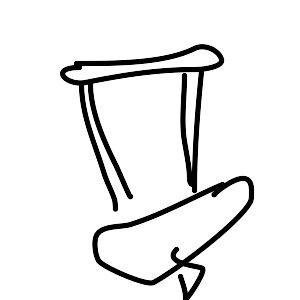
\includegraphics[width=\linewidth]{figures/fig_a.png}
\caption{Stimuli} \label{fig:1a}
\end{subfigure}
\hspace*{\fill}
\begin{subfigure}{0.23\textwidth}
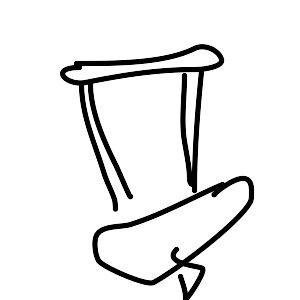
\includegraphics[width=\linewidth]{figures/fig_b.png}
\caption{Sketcher / Viewer interface} \label{fig:1b}
\end{subfigure}
\end{figure}

\subsubsection{Task} 

%% Trial-level event structure
% Drawings were collected in the context of an online, sketching-based reference game using the framework described in \citeA{Hawkins15_RealTimeWebExperiments}. 
% The game involved two players: a \textit{sketcher} who aims to help a \textit{viewer} pick out a target object from a set of distractor objects by representing it in a sketch. 
On each trial, both participants were shown the same set of four objects; however, the positions of these objects were randomized for each participant. 
One of the four objects was highlighted on the sketcher's screen to designate it as the target.
%% Trial-level objective of sketcher and viewer
Sketchers drew using black ink on digital canvas (pen width = 5 pixels; 300 $\times$ 300 pixels) embedded in a web browser window. 
Participants drew using the mouse cursor, and were not able to delete previous strokes. 
Each stroke was rendered on the viewer's screen immediately upon the completion of each stroke.
The sketcher was instructed to take no longer than 30 seconds to produce their drawings. 
The viewer was allowed guess the identity of the drawn object by clicking one of the four objects in the array as soon as they were confident. 
Both participants received immediate feedback: the sketcher learned when and which object the viewer had clicked, and the viewer learned the true identity of the target. 
Otherwise, the viewer had no other means of communicating with the sketcher. 
Both participants earned an accuracy bonus for each correct response. 
If the correct response was made under the 30-second time limit, they also received a speed bonus inversely proportional to the time taken until the response.

%% Two conditions: repeated and control

% Each pair of participants was randomly assigned two of these categories, and only the 16 objects from these two categories appeared as drawing targets during their session.

\subsubsection{Design \& Procedure} 

Each pair of participants was randomly assigned two sets of four objects: one set was was assigned to the repeated condition; the other to the control condition.
To explore how specific the effects of repeated communication were to the repeated objects, we varied the perceptual similarity between the two sets across pairs of participants. 
In half of the pairs (N=XX pairs), the repeated set contained four randomly sampled objects from one category and the control set contained the remaining four objects from the same category. 
% These control objects were thus maximally perceptually similar to the repeated objects but were not repeatedly drawn and provided a tight baseline for object-specific effects. 
In the other half of pairs (N=XX pairs), the repeated set contained four randomly sampled objects from one category and the control set contained four randomly sampled objects from the other category.
% These control objects still shared many perceptual features with the repeated objects, but provided a measure of the more generic effects of task practice. 

% The assignment of each set to the repeated and control conditions was randomized across pairs. 

The communication task consisted of three phases. 
During the \textit{repeated} phase, the sketcher drew the four repeated objects six times each, in an interleaved order.
Within this phase were six repetition cycles wherein each repeated object served as the target exactly once, and object order was randomized across repetition cycles. 
Before and after the \textit{repeated} phase, the sketcher drew all eight objects one time each, again in randomly interleaved order. 

% Including the control condition in this pre-post design allowed us to assess the specificity of repetition effects: control objects from the same category were maximally perceptually similar to the repeated objects but were not repeatedly drawn, and control objects from the other object category provided a measure of the generic effects of production task practice. 

\subsection{Results}

\begin{figure}
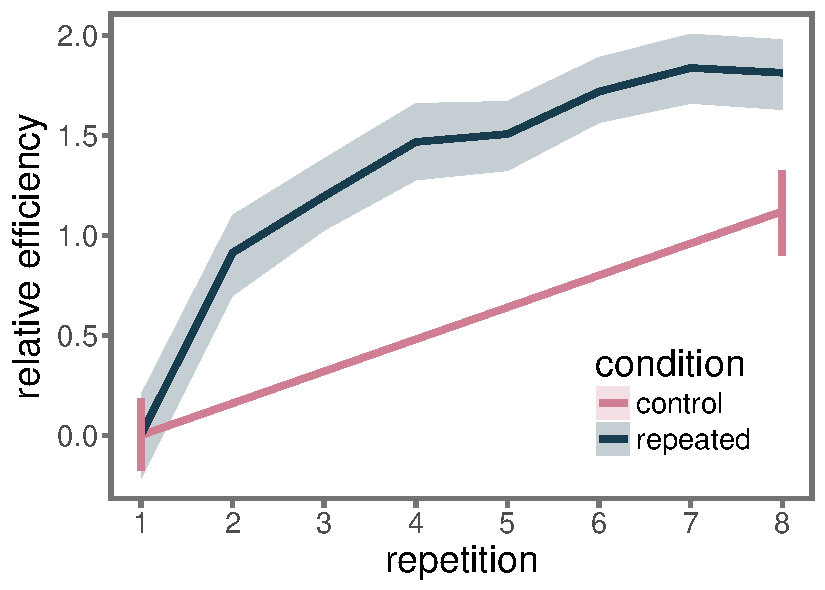
\includegraphics[width=\linewidth]{figures/refgame_BIS_timeseries.pdf}
\caption{Communication efficiency for repeated and control objects across repetitions. Efficiency was computed using a metric that combines both speed and accuracy, and is plotted relative to the first repetition.} \label{refgame_bis}
\end{figure}

In order to measure how well pairs communicated throughout each interaction, we employed a measure of communicative efficiency \cite<the \emph{i.e., balanced integration score,}>{Liesefeld2018} that takes both accuracy (i.e., proportion of correct viewer responses) and response time (i.e., time taken to produce each drawing) into account. 
This efficiency score is computed by first z-scoring the accuracy and response time variables to map these values to the same scale and then subtracting the standardized response time from standardized accuracy. 
It is thus highest when pairs are both fast \textit{and} accurate, and lowest when they make many errors and take a long time, \textit{relative} to their own performance on other trials. 

% Formula: bis_score ~ condition + (1 + condition | gameID)
% Fixed effects:
%              Estimate Std. Error        df t value Pr(>|t|)    
% (Intercept)  -1.14631    0.08343 146.52921 -13.740   <2e-16 ***
% condition1    0.03259    0.19709  71.10509   0.165    0.869    
% ---

Because objects were randomly assigned to the repeated and control conditions, we expected no differences in task performance in the pre phase. Indeed, a linear mixed-effects model with random slopes and intercepts for each pair of participants revealed no effect of condition ($b = 0.03, ~t = 0.165, ~p = 0.869$). Moreover, we found that pairs identified the target at rates well above chance in this phase (75.7\% repeated, 76.1\% control, chance = 25\%), suggesting that they were both engaged with the task but not at ceiling performance.

% Formula: bis_score ~ phase * condition + (1 + phase * condition | gameID)
%    Data: input
% Fixed effects:
%                    Estimate Std. Error        df t value Pr(>|t|)    
% (Intercept)        -0.42302    0.05473 125.82978  -7.730 2.97e-12 ***
% phase1             -1.44656    0.10112 137.22562 -14.306  < 2e-16 ***
% condition1          0.35670    0.14118  70.83601   2.527  0.01376 *  
% phase1:condition1  -0.64821    0.20974  94.62722  -3.091  0.00262 ** 
% ---
% Signif. codes:  0 ‘***’ 0.001 ‘**’ 0.01 ‘*’ 0.05 ‘.’ 0.1 ‘ ’ 1

To evaluate changes in communicative efficiency across each interaction, we fit our data with a linear mixed-effects model with maximal random effect structure, including random intercepts, slopes, and interactions for each pair of participants. 
We found that communicative efficiency increased overall between the \textit{pre} and \textit{post} phases ($b = 1.45,~t = 14.3,~p <0.001$), reflecting generalized improvements as a consequence of extended interaction.
Critically, this analysis also revealed a reliable interaction between phase and condition: communicative efficiency improved to a greater extent for repeated objects than control objects ($b = 0.648, ~t = 3.09,~p = 0.003$; see Figure \ref{refgame_bis}). 
These results show that there are benefits of repeatedly communicating about an object that accrue specifically to that object, suggesting the formation of object-specific graphical conventions. 
 
% the benefits of repeatedly communicating about an object accrue more strongly to that object 
% show gains in communicative efficiency are to some extent specific to the objects that were repeatedly referenced

% Optional: We found a similar pattern of results when we used the number of strokes in each sketch instead of drawing time in our estimate of communicative efficiency. 

% Thus, participants converged on simpler, faster, and more communicatively successful graphical conventions for repeated objects, which only partially transferred to other objects.

%We clearly see that while the cost of sketching decreases, the accuracy of the viewer's guess of which object the sketch is referring to increases, suggesting that this reduction is meaningful.

%% task-level and object-level benefits of extended communication. 

%Successful communication was primarily quantified as the viewer's accuracy in identifying the target. 
%The investment of time was measured as the length of time between the beginning of the first stroke to the completion of the final stroke in each sketch, and the investment of ink was measured in two ways: as the number of strokes used for each sketch and the proportion of the drawing canvas filled by ink.

%This ensures that the reduction in the drawing duration and number of strokes over time is not due to the players losing interest or becoming less motivated during the game. 

\section{Part II: What explains gains in communication efficiency?}

The visual communication experiment established that pairs of participants coordinate on object-specific ways of depicting objects more efficiently across repetitions.  
This raises the question: to what extent do these gains in communication efficiency reflect the accumulation of interaction-specific shared knowledge between a sketcher and viewer, as opposed to a combination of task practice and inherent visual properties of the drawings? 
To evaluate this question, we conducted two control experiments to measure the contribution of the latter. 
In these experiments, naive participants performed a drawing recognition task in which they were presented with the final drawings from the communication experiment and guessed which of four objects it referred to. 
Their task was thus the same as the viewer's in the communication experiment, except they knew their responses were not being provided as real-time feedback to the sketcher.

% , and they made their decision based on the final drawing, rather than being able to interrupt await additional information.

\subsection{Methods: Recognition Experiment}

\subsubsection{Participants}

XXX participants completed the experiment. Data from XX participants were excluded due to inconsistent responding on catch trials.  

\subsubsection{Task, Design, \& Procedure}

%How does efficiency of graphical communication, measured by how accurately and quickly the viewer can select the target intended by the sketcher, change when we change the degree of interaction specificity? 
%Here, we define interaction specificity based on both temporal structure (path dependence) and partner specificity. 
%Therefore, we design several experiments that measure the recognizability of drawings and reaction times produced in the drawing task by third-party observers. 

On each trial, recognition participants were presented with the same set of four objects and drawing viewers had in the communication game. 
Just as the viewers had been, they received an accuracy bonus for every correct response, and speed bonus inversely proportional to their response time. 

Participants were randomly assigned to two groups: a \textit{yoked} group and a \textit{shuffled} group. 
Participants in the yoked group were matched with a pair from the communication experiment and viewed 40 drawings in the same sequence the original viewer had. 
Participants in the shuffled group, on the other hand, were matched with 10 distinct pairs from the communication experiment and viewed 4 drawings from each in turn, which appeared on the same trial number as they had appeared originally. 
At the trial level, both groups thus received exactly the same visual information and performed the task under the same incentives to respond quickly and accurately. 
At the session level, both groups received exactly the same amount of practice recognizing drawings.

\subsection{Result: yoked similar to reference game}

The only difference was the inability to give feedback to the Sketcher.
% Thus, if the Sketcher does not know which object the third-party viewer had guessed on each trial. 


% Linear mixed model fit by REML. t-tests use Satterthwaite's method ['lmerModLmerTest']
% Formula: bis_relative ~ version * repetition + (1 + repetition | orig_gameID)
%    Data: d.recog %>% filter(version %in% c("communication", "yoked"))
% Fixed effects:
%                           Estimate Std. Error         df t value Pr(>|t|)    
% (Intercept)                0.44820    0.07178  274.15995   6.244 1.62e-09 ***
% versionyoked              -0.03155    0.07859 5456.46039  -0.401  0.68810    
% repetition                 0.23067    0.01706  281.10825  13.524  < 2e-16 ***
% versionyoked:repetition   -0.04999    0.01878 5457.35452  -2.661  0.00781 ** 
% ---
% Signif. codes:  0 ‘***’ 0.001 ‘**’ 0.01 ‘*’ 0.05 ‘.’ 0.1 ‘ ’ 1


\subsection{Result: conventions are interaction-specific}

% Linear mixed model fit by REML. t-tests use Satterthwaite's method ['lmerModLmerTest']
% Formula: bis_relative ~ version * repetition + (1 + repetition | gameID)
%    Data: d.recog %>% filter(version %in% c("yoked", "shuffled"))

% Fixed effects:
%                             Estimate Std. Error        df t value Pr(>|t|)    
% (Intercept)                  0.43214    0.06485 287.50472   6.663 1.36e-10 ***
% versionshuffled             -0.13284    0.08954 287.50472  -1.484    0.139    
% repetition                   0.18430    0.01440 326.27439  12.801  < 2e-16 ***
% versionshuffled:repetition  -0.09715    0.01988 326.27439  -4.888 1.60e-06 ***
% ---
% Signif. codes:  0 ‘***’ 0.001 ‘**’ 0.01 ‘*’ 0.05 ‘.’ 0.1 ‘ ’ 1


Next, we compared the yoked condition against the scrambled condition using a mixed-effects model.
We found a significant difference in recognizability: while there was some improvement across repetitions in the shuffled condition, likely attributable to a practice effect, they achieved significantly worse performance than participants in the yoked condition who saw the same sketches in their original context. 


\begin{figure}
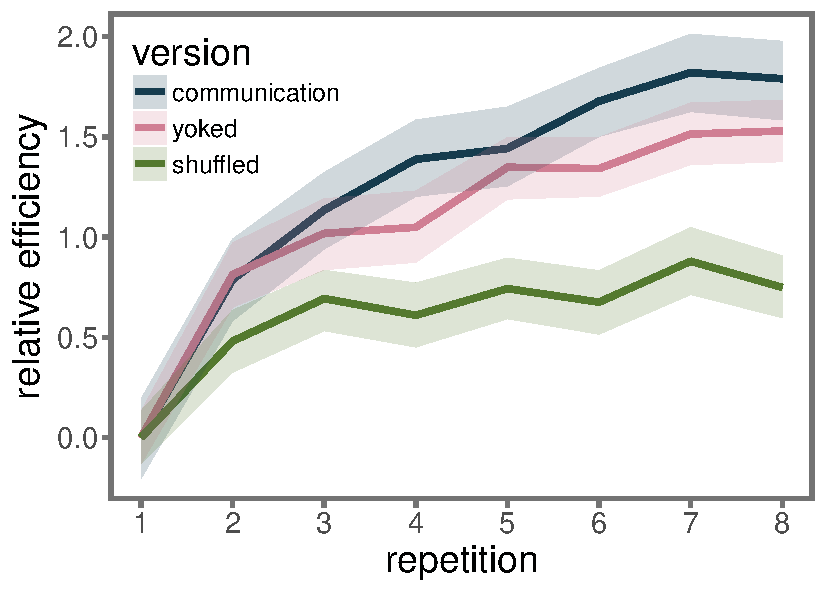
\includegraphics[width=\linewidth]{figures/recog_BIS_timeseries.pdf}
\caption{XX} \label{recog_bis}
\end{figure}

\section{Part III: How do visual features of sketches change across repetitions?}

These control experiments establish that shared history with a particular sketcher is critical for the sketches to remain meaningful late in the game. 
But what is happening over time to the visual features of the sketches themselves? 
In this final section, we conduct finer-grained analyses of the dynamics of graphical representations across communication.

First, replicating prior findings, we observed that the number of strokes used in each sketches decreased across repetitions, such that later sketches were systematically sparser than earlier ones (XXX; p < .001).

To analyze how the content of the sketches change over time, we extracted the high-level perceptual features of the drawings using a pre-trained convolutional neural network. 
Sketch features taken from the \textit{fc6} layer of VGG have been shown in prior work to match the representational space of images better than at lower layers of the network \cite{FanCommon2018}. 
In addition, features extracted from \emph{fc6} have been successful in predicting neural responses in high-level visual cortex \cite{yamins2014performance}.
We therefore define the similarity between two sketches as the correlation between their feature vectors.

\begin{figure}
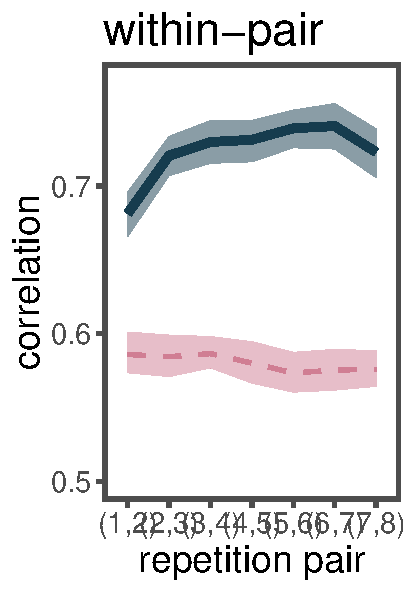
\includegraphics[width=0.45\linewidth]{figures/within.pdf}
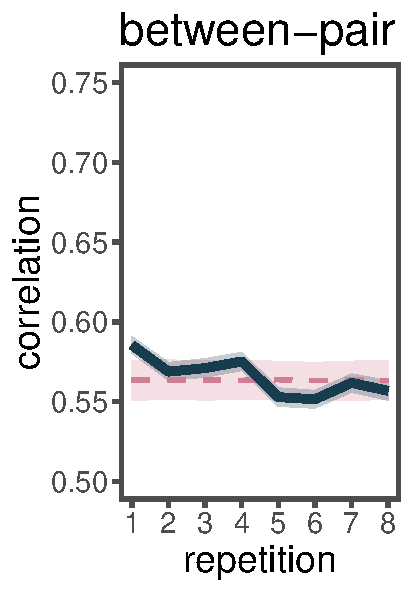
\includegraphics[width=0.45\linewidth]{figures/across.pdf}
\caption{Sketches become increasingly similar within pairs and different between pairs; error ribbons represent 95\% CI, dotted line represents permuted baseline \rdh{TODO: include insert on between-pair fig showing distribution of slopes t-scores for lmer on permuted}} \label{within-across}
\end{figure}

\subsubsection{Sketchers draw the same object more consistently across repetitions}

First, we examine the 


\subsubsection{Sketchers prioritize strokes that enhance consistency between successive sketches} 

\red{@megsano: This is the place where within-sketch lesion results can go... should be motivated by the above within-pair analysis. Stats can be on the interaction between lesion-early v. lesion-late. Exact phrasing of subheading can be further refined.}

\subsubsection{Different sketchers draw the same object differently across repetitions} 
% perhaps move this similarity explanation in the earlier subsubsection.


\subsection{Discussion}

In this paper, we XXX.
To investigate this, we used an online drawing-based reference game in which two players repeatedly communicate about visual objects, and examined both how their task performance and the drawings they produced changed over time. 
On each trial, both players were shown an array of four objects; the sketcher’s goal was to draw one of these, the target, so that the viewer could identify the target as quickly as possible. 
The game included two sets of objects: objects in one set were drawn repeatedly, while those in a control set were drawn once at the beginning and again at the end of the game. 
Across repetitions, we find that pairs discover increasingly sparse yet effective ways of depicting them. 
While we observe gains in communication efficiency for all objects, they were greater for the repeated objects, suggesting both task-level and object-level benefits of repeated communication. 
Additional control experiments revealed that these gains could not be explained by task practice alone: viewers who cycled through drawings produced by different sketchers did not improve to the same degree as viewers who were paired with a single sketcher. 
Furthermore, we found that drawings became increasingly consistent within an interaction, but that different pairs discovered different solutions for efficient communication, revealing the existence of multiple equilibria in the space of viable graphical conventions. 
Taken together, our findings suggest that repeated visual communication promotes the emergence of depictions whose meanings are increasingly determined by shared knowledge rather than their perceptual properties alone.

%\vspace{-.30cm}
\section{\bf Acknowledgments}
\small
RXDH was supported by the Stanford Graduate Fellowship and the National Science Foundation Graduate Research Fellowship (DGE-114747). NDG was supported by ONR grant N000141310341 and a Sloan Foundation fellowship.
%\vspace{-.20cm}
\bibliographystyle{apacite}

\setlength{\bibleftmargin}{.125in}
\setlength{\bibindent}{-\bibleftmargin}

\bibliography{references}


\end{document}
